\begin{figure}[t]
\centering
% src: fig/abc_views.png by scripts/paper_figures_abc.py; display parameters: docs/paper/fig_abc_provenance.json (display, views)
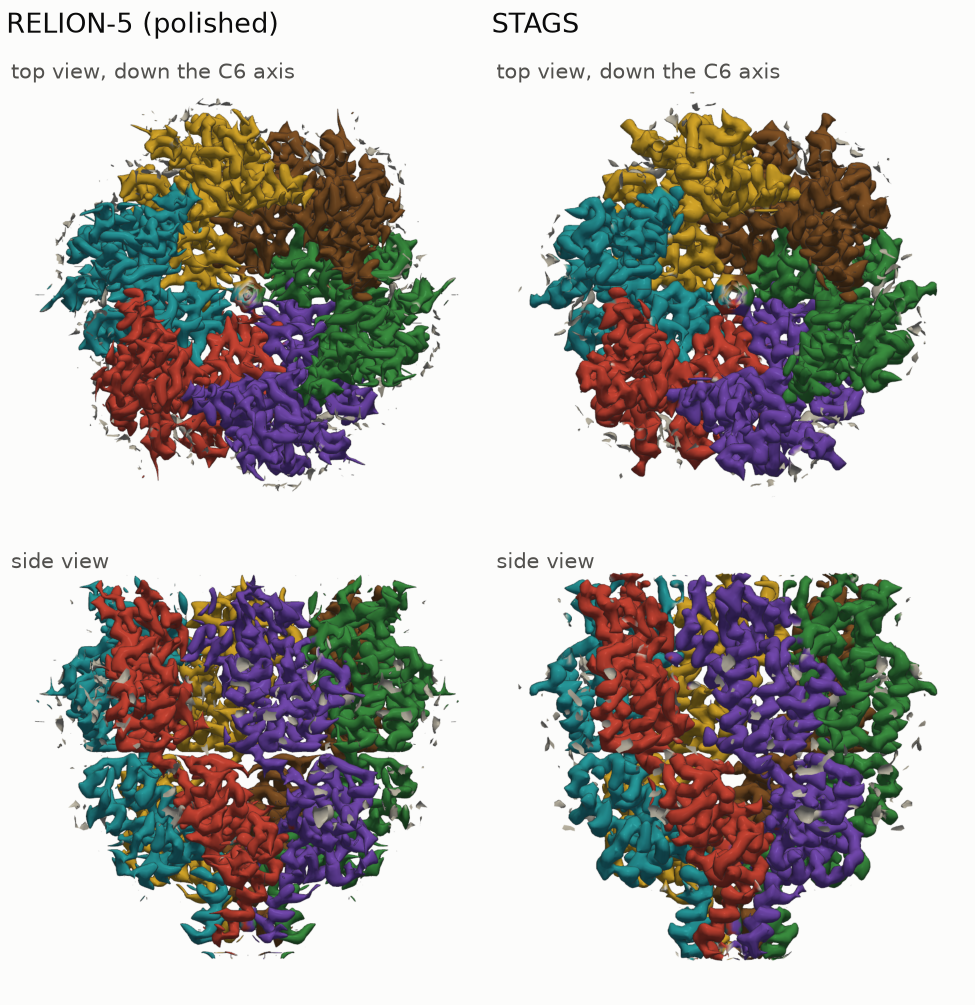
\includegraphics[width=\linewidth]{fig/abc_views.png}
\caption{\textbf{The two maps rendered identically.}
Top and side views of the central hexamer, RELION-5 polished map (left) and STAGS (right), colored by the nearest 5L93 subunit and zoned 4\,\AA\ around chains A1--A6.
Both maps: average of the two normalized half maps, the same B-factor ($-82.70$\,\AA$^2$, from RELION's post-processing job), the same raised-cosine low-pass from 3.5 to 3.1\,\AA, z-scored inside RELION's mask and thresholded to enclose the same volume, 101,942\,\AA$^3$ inside the mask (0.35$\times$ the molecular volume of the 5L93 residues inside the mask, the fraction at which RELION's map matches the silhouettes of its published Fig.~6C~\cite{burt2024relion5}); identical Taubin smoothing and cameras.}
\label{fig:views}
\end{figure}
